% modeling/transitions-DE.tex
\chapter{Übergangsfunktionen}

\section*{Motivation}
Übergänge sind der entscheidende Elementtyp der krümmungsgetriebenen
Alignment-Modellierung. Feste Elemente beschreiben geometrische Zustände
konstanter Krümmung; Übergänge beschreiben die kontrollierte Änderung zwischen
solchen Zuständen.

Im Eisenbahningenieurwesen sind Übergänge für glatte Fahrzeugbewegung, die
Begrenzung dynamischer Kräfte sowie Komfort- und Sicherheitsanforderungen
wesentlich, wie Engineering-Studien und Übersichtsliteratur zeigen
\cite{Koc2008TransitionCurves,BrustadDalmo2020Review}.

In AIM werden Übergänge nicht primär durch ihre ausdrückliche geometrische
Form, sondern durch die Entwicklung der Krümmung interpretiert.

\section{Definition durch Krümmungsentwicklung}
\begin{principle}[Prinzip der Krümmungsentwicklung]
In AIM werden Übergänge primär nach ihrer Krümmungsentwicklung und nicht nach
ihrer ausdrücklichen geometrischen Form klassifiziert.
\end{principle}
\begin{definition}[Übergang]
Ein Übergang ist ein Alignment-Element, dessen Krümmung über seinem
Parameterintervall variiert.
\end{definition}
\begin{definition}[Krümmungsgesetz eines Übergangs]
Es sei \(L>0\). Ein Krümmungsgesetz eines Übergangs ist eine Funktion
\[
\kappa:[0,L]\to\R
\]
mit vorgegebenen Randwerten
\[
\kappa(0)=\kappa_0,\qquad\kappa(L)=\kappa_1.
\]
\end{definition}
Diese Formulierung folgt unmittelbar der krümmungsbasierten Beschreibung
ebener Kurven \cite{DoCarmo1976Curves}.

\section{Normierte Darstellung}
\begin{definition}[Normiertes Übergangsgesetz]
Ein normierter Übergang wird definiert durch
\[
\widehat{\kappa}:[0,1]\to\R
\]
mit
\[
\widehat{\kappa}(0)=0,\qquad\widehat{\kappa}(1)=1.
\]
\end{definition}

Normierung trennt die geometrische Form eines Übergangs von seinem Maßstab und
ermöglicht den systematischen Vergleich von Übergangsfamilien. Sie trennt
intrinsisches Übergangsverhalten vom physischen Maßstab und ermöglicht damit
wiederverwendbare Übergangsregister und familienbasierte Modellierung.

Die folgende Vergleichsabbildung beantwortet die Engineering-Frage der
Übergangsmodellierung: Wo treten bei ähnlich erscheinenden geometrischen
Pfaden weiterhin operativ relevante Unterschiede in das Modell ein?

\begin{figure}[ht]
\centering
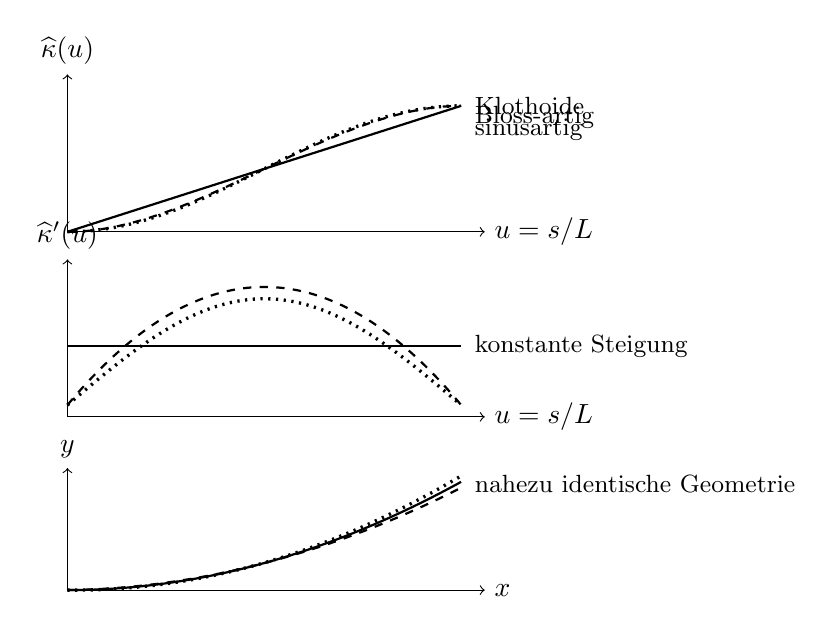
\begin{tikzpicture}[scale=1.0,axis/.style={->,thin},curve/.style={thick},label/.style={font=\small}]
\begin{scope}[shift={(0,4.0)}]
\draw[axis] (0,0)--(5.3,0) node[right] {$u=s/L$};
\draw[axis] (0,0)--(0,2.0) node[above] {$\widehat{\kappa}(u)$};
\draw[curve] plot[smooth,domain=0:5,samples=40] (\x,{0.32*\x});
\draw[curve,dashed] plot[smooth,domain=0:5,samples=80] (\x,{1.6*(3*(\x/5)^2-2*(\x/5)^3)});
\draw[curve,dotted,very thick] plot[smooth,domain=0:5,samples=80] (\x,{1.6*(0.5-0.5*cos(180*\x/5))});
\node[label,right] at (5.05,1.60) {Klothoide};
\node[label,right] at (5.05,1.45) {Bloss-artig};
\node[label,right] at (5.05,1.30) {sinusartig};
\end{scope}
\begin{scope}[shift={(0,1.65)}]
\draw[axis] (0,0)--(5.3,0) node[right] {$u=s/L$};
\draw[axis] (0,0)--(0,2.0) node[above] {$\widehat{\kappa}'(u)$};
\draw[curve] (0,0.9)--(5,0.9);
\draw[curve,dashed] plot[smooth,domain=0:5,samples=80] (\x,{0.15+1.5*(6*(\x/5)-6*(\x/5)^2)/1.5});
\draw[curve,dotted,very thick] plot[smooth,domain=0:5,samples=80] (\x,{0.15+1.35*sin(180*\x/5)});
\node[label,right] at (5.05,0.90) {konstante Steigung};
\end{scope}
\begin{scope}[shift={(0,-0.55)}]
\draw[axis] (0,0)--(5.3,0) node[right] {$x$};
\draw[axis] (0,0)--(0,1.55) node[above] {$y$};
\draw[curve] plot[smooth,domain=0:5,samples=80] (\x,{0.055*\x^2});
\draw[curve,dashed] plot[smooth,domain=0:5,samples=80] (\x,{0.052*\x^2+0.018*sin(180*\x/5)});
\draw[curve,dotted,very thick] plot[smooth,domain=0:5,samples=80] (\x,{0.058*\x^2-0.015*sin(180*\x/5)});
\node[label,right] at (5.05,1.35) {nahezu identische Geometrie};
\end{scope}
\end{tikzpicture}
\caption{Übergangsfamilien können sehr ähnliche geometrische Pfade erzeugen und sich zugleich stark in Krümmungsentwicklung und Krümmungsableitungen unterscheiden. Deshalb muss Übergangsentwurf anhand von Krümmung und Dynamik und nicht nur im Ortsraum bewertet werden.}
\end{figure}

Übergänge, die im Ortsraum nahezu identisch erscheinen, können sich in den
Krümmungsableitungen und damit im dynamischen Verhalten erheblich
unterscheiden. Methodisch folgt daraus: Die Auswahl eines Übergangs kann nicht
allein durch geometrische Anpassung begründet werden; sie muss
Krümmungsentwicklung und Laufzeitkriterien auf Ableitungsebene einschließen.

\section{Skalierung}
\begin{proposition}
Sei \(\widehat{\kappa}\) ein normiertes Übergangsgesetz. Dann ist ein
physischer Übergang gegeben durch
\[
\kappa(s)=\kappa_0+(\kappa_1-\kappa_0)\,
\widehat{\kappa}\!\left(\frac{s}{L}\right).
\]
\end{proposition}
Dies trennt Form und Maßstab und begründet wiederverwendbare
Übergangsfamilien und parametrisierten Entwurf.

\section{Regularität und Glattheit}
\begin{definition}[Regularitätsklasse]
Ein Übergang gehört zur Klasse \(C^k\), wenn seine Krümmungsfunktion \(k\)-mal
stetig differenzierbar ist.
\end{definition}
In der Engineering-Praxis stehen Eigenschaften höherer Ordnung wie
Krümmungsableitungen unmittelbar mit Fahrkomfort und dynamischer Belastung in
Beziehung \cite{Mieloszyk2012Transition,Koc2017SmoothedEnds}.
\OPEN{Formale Rolle von $\kappa'$ und $\kappa''$ in Engineering-Regeln.}

\section{Übergangsfamilien}
\begin{definition}[Übergangsfamilie]
Eine Übergangsfamilie ist eine Klasse von Krümmungsgesetzen mit gemeinsamer
funktionaler Struktur.
\end{definition}

\subsection{Klassische Familien}
Der klassische Übergangsbogen im Eisenbahningenieurwesen ist die Klothoide mit
linearer Krümmungsentwicklung:
\[
\kappa(s)\propto s.
\]
Historisch lässt sich diese Entwicklung über frühe Arbeiten von Glover
\cite{Glover1900TransitionCurves}, Horsburgh
\cite{Horsburgh1913TransitionCurve} und Higgins
\cite{Higgins1922TransitionSpiral} verfolgen.

\subsection{Polynomiale und alternative Familien}
Polynomiale Übergangsbögen bieten zusätzliche Freiheit bei der Formung von
Krümmungsentwicklung und Ableitungen. Solche Ansätze sind mit moderner
Forschung zu polynomialer Glättung \cite{ZboinskiWoznica2017Polynomial} und
den regelungsorientierten Konstruktionen von Klauder
\cite{Klauder2001BetterWay,Klauder2009US} verbunden.
\TODO{Formale Definition polynomialer Übergangsfamilien.}

\subsection{Geometrische Familien}
Manche Übergangsbögen werden durch geometrische oder implizite Beziehungen
statt durch ausdrückliche Krümmungsgesetze eingeführt.
\begin{example}
Lemniskatenartige oder sinusbezogene Konstruktionen gehören nach geeigneter
Reparametrisierung in den Krümmungsraum zu dieser Klasse
\cite{Pirti2016Transrapid}.
\end{example}
Vor ihrer Integration in den vorliegenden Rahmen müssen diese Kurven in eine
\(\kappa(s)\)-Darstellung überführt werden.

\subsection{Engineering- und praxisorientierte Familien}
Die Engineering-Praxis führt Übergangsbögen häufig durch Entwurfsregeln und
operative Erwägungen statt durch rein theoretische Herleitung ein. Der
Bloss-Übergang ist ein wichtiges Beispiel einer praktischen Engineering-Familie,
ursprünglich beschrieben von Bloss \cite{Bloss1978TrackGeometry} und in
modernen Übersichten weiter erörtert \cite{Ciobanu2015Bloss}.

\subsection{Moderne und hybride Familien}
Die moderne Engineering-Praxis betrachtet zahlreiche Übergangsfamilien mit
verbessertem dynamischem Verhalten, glatteren Endeigenschaften oder Regelung
höherer Ordnung. Beispiele sind Übergänge mit geglätteter Krümmung nach Koc
\cite{Koc2017SmoothedEnds,Koc2019SmoothedTransition,Koc2019Operational} und
Ansätze zum Wiener Bogen \cite{Wojtczak2017WienerBogen}.
\RESEARCH{Systematische Klassifikation moderner Übergangsfamilien.}

\section{Zerlegungsansätze}
Ein Übergang muss nicht stets als unteilbares Objekt behandelt werden. Seine
Darstellung als Komposition von Unterelementen kann nützlich sein.

Das in \cref{sec:berlinish-composition} eingeführte Berlinish-Framework liefert
die konkrete Zerlegung
\[
T=H_{\mathrm{in}}+C+H_{\mathrm{out}},
\qquad
L_{H_{\mathrm{in}}},L_C,L_{H_{\mathrm{out}}}\geq 0.
\]
Es ist eine mathematische Kompositionsgrammatik: Komponentenlängen null und die
Wahl der Halbwellenfunktionen bestimmen reine, einseitige, asymmetrische und
zusammengesetzte Fälle. Eine dünn besetzte Implementierung kann dieselbe
Grammatik durch Familienkennung, normierte Teilungen, Funktionsreferenzen und
Parameter kodieren. Mathematische Interpretation und konkrete Datenkodierung
sind miteinander verbunden, aber nicht identisch.

\section{Operatorsicht}
\begin{principle}[Prinzip des Übergangsoperators]
Ein Übergangselement wirkt als lokaler Operator der Krümmungsentwicklung, der
einen geometrischen Zustand in einen anderen transformiert.
\end{principle}
Übergänge können damit als Operatoren der Zustandsentwicklung statt bloß als
vordefinierte geometrische Kurvenformen interpretiert werden.
\RESEARCH{Formale Operatoralgebra der Übergänge.}

\section{Implementierungssicht}
In rechnerischen Systemen können Übergangsbögen dargestellt werden durch:
\begin{itemize}
\item analytische Ausdrücke,
\item polynomiale Approximationen,
\item Nachschlagetabellen und
\item kompilierte hybride Darstellungen.
\end{itemize}
Übergangsfamilien können durch Register normierter Krümmungsgesetze mit
Ableitungs- und Integrationsoperatoren dargestellt werden.

In der ursprünglichen Systemlinie bezeichnet \emph{transitionDB} die
strukturierte Wissensbasis aus Funktionsidentitäten, Halbwellenfamilien,
Parametern und bekannten Übergangsformen. Die aktuelle
Referenzimplementierung realisiert einen wesentlichen Teil dieser Rolle durch
eine validierte Transition-Registry: Sie enthält normierte
Prototypfunktionen, Halbwellenbeschreibungen, Familienteilungen und benannte
Übergangseinträge. Dies ist Implementierungsevidenz für den
Kompositionsmechanismus, aber kein Beleg dafür, dass jede historische oder
proprietäre Form erfasst ist.

\emph{TransEd} ist der zugehörige Untersuchungs- und Bearbeitungsarbeitsraum.
Sein Zweck ist die Prüfung normierter Krümmungs- und Ableitungsverläufe sowie
die Arbeit mit wiederverwendbaren Übergangsdefinitionen; TransEd besitzt weder
Alignment Identity noch ersetzt es die Bearbeitung auf Alignment-Ebene.
Analytische Ausdrücke und Nachschlagerepräsentationen bleiben alternative
Realisierungen eines Funktionsgesetzes mit der üblichen Abwägung zwischen
nachvollziehbarer exakter Struktur und Laufzeiteffizienz.

\section{Bezug zum Eisenbahningenieurwesen}
In Eisenbahnanwendungen sind Übergänge eng mit operativen Parametern wie
Geschwindigkeit und Überhöhung gekoppelt und müssen strenge
Engineering-Bedingungen erfüllen
\cite{Kufver2000RailwayAlignment,Klein1998Trassierung}.
Die Übersichtsliteratur bestätigt, dass Übergangsbögen nicht nur geometrisch,
sondern auch hinsichtlich Komfort, Instandhaltung und dynamischer Reaktion zu
verstehen sind \cite{BrustadDalmo2020Review}.

\section{Zusammenfassung}
\begin{summary}
Übergänge definieren die kontrollierte Entwicklung der Krümmung zwischen
geometrischen Zuständen.

In AIM werden sie als normierte Operatoren der Krümmungsentwicklung und nicht
lediglich als vordefinierte geometrische Kurventypen interpretiert.

Ihre normierte Darstellung ermöglicht wiederverwendbare Übergangsfamilien,
operatorbasierte Modellierung und die Laufzeitrekonstruktion von
Alignment-Geometrie und -Dynamik.
\end{summary}
